% IDEA: separate theoretical/general approach and concrete decisions
% this means, for example, that:
% PART1:
% - requirements for lifted functions, soundness
% - implication (gradual, ...)
% - abstract versions of [w/o], append
% PART2:
% - concrete version of [w/o], append, ... (probably requires notion of normalized env :( )
% - actual implementation

\chapter{Introduction}
Most modern programming languages use static analysis to some degree, ruling out certain types of runtime failure.
Static analysis provides guarantees about the dynamic behavior of a program without actually running the program.
%% static typing
Static typing disciplines are among the most common representatives of static analysis, guaranteeing type safety at compile time, obviating the need for dynamic checks.

%% static verification
Another powerful technique is static verification of programs against their specification, i.e. statically proving their “correctness”.
In practice this is achieved by checking that some annotated invariants or assertions (reflecting the specification) must always hold.
% example?
Unfortunately, static verification has limitations and drawbacks:
\begin{itemize} % TODO
    \item Syntax
    \item Decidability
    \item Difficult and Tedious to annotate programs
    \item ...
\end{itemize}
These limitations not only affect programmers trying to statically verify their program.
Most general purpose programming languages (C/C++, C\#, Java, ...), usually driven by cost-benefit and usability considerations, haven't adopted this level of static analysis in the first place.

%% grad verification
The purpose of gradual verification is to weaken if not remove some of these limitations at the cost of turning some static checks into runtime checks, whenever inevitable.
We will present a procedure of turning a static verification into a gradual one.
% more detail about static limitations and how runtime circumvents them?

%% static typing weakened
This idea is not new at all and actually common practice in type systems:
In C\# or Java, explicit type casts are assertions about the actual type of a value.
This actual type (usually a subtype of the statically known type) could not be deduced by the static type system due to its limitations.
Such an assertion/cast allows subsequent static reasoning about the value assuming its new type at the cost of an additional runtime check, ensuring the validity of the cast.
Note that such deviations from a “purely” static type system (one where there is no need for runtime checks) do not affect type safety:
It is still guaranteed that execution does not enter an invalid state (one where runtime types are incompatible with statically annotated types) by simply interrupting execution whenever a runtime type check fails.
This is usually implemented by throwing an exception.
% mention that runtime cost reasonable, ...


%% dyn typing
At the other end of the spectrum are dynamically typed languages.
In scenarios where the limitations of a static type system would clutter up the source code, they allow expressing the same logic with less syntactic overhead, but at the cost of less static guarantees and early bug detection.

%% PLs are on the dynamic end of the verification spectrum
In terms of program verification, most general purpose languages are on the dynamic end of the spectrum.
If they exist as designated syntax, assertions are usually implemented as runtime checks and often even dropped entirely for “release” builds (the Java compiler drops them by default).
It is common practice to implement 
% research Eiffel!
% Design-by-Contract!!! Eiffel!
% D even has both

% this is more of a consequence of the “deep roots” of dynamic verification!!!
%But even preconditions at expression level are implemented as runtime checks, reflected all the way down at instruction architecture level.
%Examples:
%\begin{description}
%    \item[Division by zero]~\\
%    Integer division performs a dynamic check...
%    
%\end{description}

%% grad typing
A gradual type system is more flexible, as it provides the full continuum between static and dynamic typing, letting the programmer decide ... %TODO.
It can be seen as an extension  “unknown” type 


This work will also show that gradual verification ... other angle!

- 
What is the thesis about?
Why is it relevant or important?
What are the issues or problems?
What is the proposed solution or approach?
What can one expect in the rest of the thesis?

“Static verification checks that properties are always true, but it can be difficult and tedious to select a goal and to annotate programs for input to a static checker.” (http://www.sciencedirect.com/science/article/pii/S1571066104002567)


\section{Motivation}
more practical view? Intro? Background?



\chapter{Background}

\section{Categorization of existing stuff}
\cite{arlt2014gradual}
GraVy:
metric of progress of the verification process
and allows the verification engineer to focus on the remaining statements.
Gradual verification is not a new static verification technique. It is an extension
that can be applied to any existing static verification techniques to provide
additional information to the verification engineer. Thus, issues, such as handling
of loops or aliasing are not addressed in this paper. These are problems
related to sound verification, but gradual verification is about how to make the
use of such verification more traceable and quantifiable

\cite{nelson2004extended} ESC/Java
Software development and maintenance are costly endeavors.
The cost can be reduced if more software defects are
detected earlier in the development cycle. This paper introduces
the Extended Static Checker for Java (ESC/Java),
an experimental compile-time program checker that finds
common programming errors. The checker is powered by
verification-condition generation and automatic theorem proving
techniques. It provides programmers with a simple
annotation language with which programmer design decisions
can be expressed formally. ESC/Java examines the
annotated software and warns of inconsistencies between the
design decisions recorded in the annotations and the actual
code, and also warns of potential runtime errors in the code.
This paper gives an overview of the checker architecture and
annotation language and describes our experience applying
the checker to tens of thousands of lines of Java programs.

\cite{jacobs2001logic} JML => static verification

\cite{cheon2002runtime} JML => RAC

\cite{the-spec-programming-system-an-overview} Spec\#

\cite{a-statically-verifiable-programming-model-for-concurrent-object-oriented-programs} Spec\# extension (concurrent OO)

\cite{meyer2002design} Design-by-Contract
then also: Eiffel by Bertrand Meyer 

\cite{embedded-contract-languages} Code Contracts! Combines runtime and static checking

\cite{crocker2004safe} “verified design-by-contract”

\cite{ChristakisMuellerWuestholz16}
= static verification plus directed dynamic verification
In this paper, we present a technique to complement partial
verification results by automatic test case generation. In
contrast to existing work, our technique supports the common
case that the verification results are based on unsound
assumptions. We annotate programs to reflect which executions
have been verified, and under which assumptions.
These annotations are then used to guide dynamic symbolic
execution toward unverified program executions. Our main
technical contribution is a code instrumentation that causes
dynamic symbolic execution to abort tests that lead to verified
executions, to prune parts of the search space, and to
prioritize tests that cover more properties that are not fully
verified.

\section{Hoare Logic}
...for static semantics

\cite{hoare1969axiomatic}

\section{Related Work}
\subsection{Abstracting Gradual Typing}
\cite{siek2006gradual}
Gradual Typing for Functional Languages

apply their gradual typing approach to other areas

\cite{siek2015refined}
Refined criteria for gradual typing
gradual guarantee:
     The gradual guarantee says that if a gradually typed program is
     well typed, then removing type annotations always produces a program that is still well typed.
     Further, if a gradually typed program evaluates to a value, then removing type annotations
     always produces a program that evaluates to an equivalent value.

\cite{garcia2016abstracting}
AGT
In this paper, we propose a new formal foundation for gradual
typing, drawing on principles from abstract interpretation to
give gradual types a semantics in terms of preexisting static types.
Abstracting Gradual Typing (AGT for short) yields a formal account
of consistency—one of the cornerstones of the gradual typing
approach—that subsumes existing notions of consistency, which
were developed through intuition and ad hoc reasoning.

\cite{garcia2015deriving}
Abstracting Gradual Typing (AGT) is an approach to systematically
deriving gradual counterparts to static type disciplines (Garcia
et al. 2016). The approach consists of defining the semantics of
gradual types by interpreting them as sets of static types, and then
defining an optimal abstraction back to gradual types. These operations
are used to lift the static discipline to the gradual setting. The
runtime semantics of the gradual language then arises as reductions
on gradual typing derivations.
To demonstrate the flexibility of AGT, we gradualize
a prototypical security-typed language
with respect to only security labels rather than entire types, yielding
a type system that ranges gradually from simply-typed to securely typed.
We establish noninterference for our gradual language using Zdancewic’s logical relation proof method.
Whereas prior work presents gradual security cast languages,
which require explicit security casts, this work yields the first gradual
security source language, which requires no explicit casts.

prior to AGT
\cite{wolff2011gradual}
the language extends the notion of gradual typing to account for typestate: gradual typestate
checking seamlessly combines static and dynamic checking by automatically
inserting runtime checks into programs.

\cite{banados2014theory}
 develop a theory of gradual effect checking, which
 makes it possible to incrementally annotate and statically check
 effects, while still rejecting statically inconsistent programs. We
 extend the generic type-and-effect framework of Marino and Millstein
 with a notion of unknown effects, which turns out to be significantly
 more subtle than unknown types in traditional gradual
 typing. We appeal to abstract interpretation to develop and validate
 the concepts of gradual effect checking.

\cite{toro2015customizable}
Grad Effects in Scala, benchmarks on runtime impact!

\subsection{Implicit Dynamic Frames}

Race-free Assertion language! => static verification tool able to reason soundly about concurrent programs

% separating conjuction (= Multiplicative conjunction ⊗, lollipop, ...), access is resource, cannot duplicate access, ...
% TODO: explain Frame Problem
% translation of separating conjuction to regular conjunction? would simplify later reasoning A LOT

\cite{smans2009implicit}
IDF


\cite{leino2009verification}
Chalice, a verification methodology based on implicit dynamic frames

Chalice’s verification methodology centers around permissions and permission transfer. In particular, a memory location may be accessed by a thread only if that thread has permission to do so. Proper use of permissions allows Chalice to deduce upper bounds on the set of locations modifiable by a method and guarantees the absence of data races for concurrent programs. The lecture notes informally explain how Chalice works through various examples.

also: Viper (Verification Infrastructure for Permission-based Reasoning; is a suite of tools developed at ETH Zurich, providing an architecture on which new verification tools and prototypes can be developed simply and quickly.) has Chalice as front-end

\cite{summers2013formal}
In this paper, we provide both an isorecursive and an equirecursive formal
semantics for recursive definitions in the context of Chalice

\cite{parkinson2011relationship}
VERY IMPORTANT: chapter 2.2

Finally, we show that we can encode the separation
logic fragment of our logic into the implicit dynamic frames fragment, preserving
semantics. For the connectives typically supported by tools, this shows that separation
logic can be faithfully encoded in a first-order automatic verification tool (Chalice).

Although IDF was partially inspired by separation logic, there are many differences
between SL and IDF that make understanding their relationship difficult. SL does not
allow expressions that refer to the heap, while IDF does. SL is defined on partial heaps,
while IDF is defined using total heaps and permission masks. The semantics of IDF are only defined by its translation to first-order verification conditions, while SL has a direct
Kripke semantics for its assertions.

\subsubsection{Self-Framing}



%STRUCTURE:
% - intruduce static sample language (interesting for IDF, blabla, ..., but also general enough to transfer ideas)
% - gradualize sample language without focus on impl. details (assume NPC/undec. sat, impl, ... to stay general), i.e. focus on principal correctness        (undecidable in general => SMT solvers)
% - implement this very language and show effects of precision, ...


\chapter{Gradualization of a Statically Verified Language}
%% why start with static language
As illustrated earlier %MAKE SURE!
gradual verification can be seen as an extension of both static and dynamic verification.
% Both can be seen as the endpoints of the continuum...?
Yet, our approach of “gradualization” formalizes the introduction of the dynamic aspect into a fully static system.
Thus, this %TODO: work, section, chapter?
uses a statically verified language as starting point.
Later %TODO: ref
we will show how a programming language without static verification can be approached.

%% more about our language
We will now intrude a very simple Java-like language that uses Chalice/Eiffel/Spec\# %???
 sub-syntax to express method contracts.
% more about simplicity?

%% structure of this chapter
% TODO

\section{A Statically Verified Language}
\label{sec:a-statically-verified}
\begin{comment}
    \begin{alignat*}{3}
    	 & \rlap{\textbf{Syntax}}                        &  &                      & ~ \\
    	 & s                                             &  & \in \setStmt         &  \\
    	 & \phi                                          &  & \in \setFormula      &  \\
    	 &  \\
    	 & \rlap{\textbf{Program State}}                 &  &                      &  \\
    	 & \pi                                           &  & \in \setProgramState &  \\
    	 &  \\
    	 & \rlap{\textbf{Semantics}}                     &  &                      &  \\
    	 & \rlap{Static  ~~~~$\thoare{}{\phi}{s}{\phi}$} &  &                      &  \\
    	 & \rlap{Dynamic ~$\sstep{\pi}{\pi}$}            &  &                      &  \\
    	 & \rlap{Formula ~~$\evalphiGen{\pi}{\phi}$}     &  &                      &  \\
         & ~ \\
         & \rlap{\textbf{Soundness}}                     &  &                      &  \\
    \end{alignat*}

    \begin{alignat*}{3}
    	 & \rlap{\textbf{Syntax}}                                              &  &                       & ~ \\
    	 & \grad{s}                                                            &  & \in \setGStmt         &  \\
    	 & \grad{\phi}                                                         &  & \in \setGFormula      &  \\
    	 &  \\
    	 & \rlap{\textbf{Program State}}                                       &  &                       &  \\
    	 & \grad{\pi}                                                          &  & \in \setGProgramState &  \\
    	 &  \\
    	 & \rlap{\textbf{Semantics}}                                           &  &                       &  \\
    	 & \rlap{Static  ~~~~$\gthoare{}{\grad{\phi}}{\grad{s}}{\grad{\phi}}$} &  &                       &  \\
    	 & \rlap{Dynamic ~$\gsstep{\grad{\pi}}{\grad{\pi}}$}                   &  &                       &  \\
    	 & \rlap{Formula ~~$\evalgphiGen{\grad{\pi}}{\grad{\phi}}$}            &  &                       &  \\
    	 & ~ \\
    	 & \rlap{\textbf{Soundness}}                                           &  &                       &
    \end{alignat*}
\end{comment}



%% generic language introduction
While aiming to give a general procedure for deriving imperative gradually verified languages, we have to make certain assumptions about \svl in order to concisely describe our approach and reason about its correctness.
We believe that most imperative statically verified programming languages satisfy the following assumptions and thus qualify as starting point for our procedure.

\begin{description}
\item[Syntax]~\\
    We assume the existence of the following two syntactic categories:
    \begin{align*}
    	s    & \in \setStmt    \\
    	\phi & \in \setFormula
    \end{align*}
    
    We assume that there is a sequence operator \ttt{;} such that $$\forall s_1, s_2 \in \setStmt.~~ s_1\ttt{;}s_2 \in \setStmt$$
    
\item[Program State]~\\
    Dynamic semantics (see below) are formalized as discrete transitions between program states.
    Therefore a program state contains all information necessary to evaluate expressions and determine the next program state.
    We assume that $\setProgramState$ is the set of all possible program states in \svl.
    
    \begin{example}{Program State: Primitive language with integer variables}
        \label{ex:ps-primitive}
        \begin{displaymath}
        \setProgramState ~=~ \underbrace{(\setVar \rightharpoonup \mathbb{Z})}_{\textit{variable memory}} ~\times~ \setStmt 
        \end{displaymath}
    \end{example}
    \begin{example}{Program State: Language with stack}
        \label{ex:ps-stacked}
        \begin{displaymath}
        \setProgramState ~=~ \bigcup_{i \in \mathbb{N}_+}{\underbrace{\Big((\setVar \rightharpoonup \mathbb{Z}) ~\times~ \setStmt \Big)}_{\textit{stack frame}}}^i                                                      
        \end{displaymath}
    \end{example}
    
    Note how these examples use statements to represent continuations (the “remaining work”), necessary for the operational semantics to deduce a state transition.
    In general, a different representation may be used to encode this continuation (e.g. a lower-level machine language emitted by the compiler).
    
    \begin{comment}
    In order to determine the next program state (or detect termination), a state must have a notion of “upcoming work”, usually represented by a statement internally.
    
    Let $\setProgramState_s$ (with $s \in \setStmt$) be the set of program states having $s$ as upcoming work.
    This notion will be necessary to define soundness of \svl's static semantics.
    
    Examples:
    \begin{description}
        \item[Primitive]
        \begin{flalign*}
        	 & \setProgramState ~=~ \underbrace{(\setVar \rightharpoonup \mathbb{Z})}_{\textit{variable memory}} ~\times~ \setStmt & ~ \\
        	 & \setProgramState_s ~=~ (\setVar \rightharpoonup \mathbb{Z}) ~\times~ \setStmt_s                                     &
        \end{flalign*}
        
        \item[Stack]
        \begin{flalign*}
        	 & \setProgramState ~=~ \bigcup_{i \in \mathbb{N}_+}{\underbrace{\Big((\setVar \rightharpoonup \mathbb{Z}) ~\times~ \setStmt \Big)}_{\textit{stack frame}}}^i                                                                                \\
        	 & \setProgramState_s ~=~ \Big((\setVar \rightharpoonup \mathbb{Z}) ~\times~ \setStmt_s\Big) ~\times~ \underbrace{\bigcup_{i \in \mathbb{N}_0}{\Big((\setVar \rightharpoonup \mathbb{Z}) ~\times~ \setStmt \Big)^i}}_{\textit{lower frames}}
        \end{flalign*}
    \end{description}
     
    \end{comment}
    
    
\item[Dynamic Semantics]~\\
    We assume that \svl has a structural operational semantics or small-step semantics.
    This semantics is formalized as $~\sstep{\cdot}{\cdot} : \setProgramState \rightharpoonup \setProgramState$, describing precisely how program state can be updated. % TODO: reconsider non-deterministic
    %We assume that there is a small-step semantics $~\sssem \subseteq \setProgramState \rightarrow \PP(\setProgramState)$ describing precisely how program state can be updated.
    %Note that this signature allows for non-deterministic (e.g. concurrent) semantics.
    %Execution is considered stuck in state $\pi$ iff $\sssem(\pi) = \emptyset$
    As usual, 
    %taking $n$ steps is abbreviated as $\sstepGeneric{\cdot}{n}{\cdot}$ (undefinedness is propagated), 
    taking a finite amount of steps is abbreviated as $\ssteps{\cdot}{\cdot}$.
    Also, we write $\sstepStuck{\pi}$ to state that $\pi$ is a “stuck” state, i.e. that $\pi$ is not in the domain of the partial small-step function.
    
    Furthermore we define $\sstepConsume{s}{\cdot}{\cdot} \subseteq \setProgramState \times \setProgramState$ as a predicate indicating whether a program state is reachable from another program state by executing statement $s$.
    This is useful for abstracting over the precise implementation of both $\setProgramState$ (see examples \ref{ex:ps-primitive} and \ref{ex:ps-stacked}) and the small-step semantics.
    
    \begin{example}{Execution of Given Statement}
        Assume that program state is defined as in example \ref{ex:ps-primitive}.
        If $\pi_1 \in \setProgramState$ is defined as
        \begin{displaymath}
        \pi_1 = \langle [x \mapsto 4, y \mapsto 2],\,\, \sSeq{\sVarAssign{x}{8}}{\sVarAssign{y}{x}} \rangle
        \end{displaymath}
        then $\sstepConsume{\sVarAssign{x}{8}}{\pi_1}{\pi_2}$ is supposed to hold for
        \begin{displaymath}
        \pi_2 = \langle [x \mapsto 8, y \mapsto 2],\,\, \sVarAssign{y}{x} \rangle
        \end{displaymath}
        
        Apparently the notation hides away the implementation details of the small-step semantics.
        It enables reasoning about small-step derivations (that correspond to executing certain statements) without worrying about the exact number of steps taken.
        
        Note that the judgment $\ssteps{\pi_1}{\pi_2}$ is also independent from the number of steps taken, yet it does not encode what is supposed to happen during those steps.
        For $\pi_1$ defined as above
        \begin{displaymath}
        \pi_2 = \langle [x \mapsto 8, y \mapsto 8],\,\, \sSkip \rangle
        \end{displaymath}
        or
        \begin{displaymath}
        \pi_2 = \pi_1
        \end{displaymath}
        would be a valid instantiations.
    \end{example}
    
    We assume that there is a designated non-empty set $~\setProgramStateFin \subseteq \setProgramState~$ of states indicating regular termination of the program.
    W.l.o.g. we assume $\forall \pi \in \setProgramStateFin.~ \sstepStuck{\pi}$, i.e. final states are stuck.
    
    We assume that dynamic semantics of a sequence $\sSeq{$s_1$}{$s_2$}$ is implemented such that 
    \begin{align}
    \label{frm:assume-seq-ss}
    \sstepConsume{\sSeq{$s_1$}{$s_2$}}{\pi_1}{\pi_3} \iff \exists \pi_2 \in \setProgramState.~ \sstepConsume{s_1}{\pi_1}{\pi_2} \wedge \sstepConsume{s_2}{\pi_2}{\pi_3}
    \end{align}
    for all $\pi_1, \pi_3 \in \setProgramState$.
    
    
    % We say a statement “throws an exception” if its small-step semantics transitions into an exceptional state.
    \begin{comment}
    Optionally, there may be a subset $~\setProgramStateEx \subseteq \setProgramStateFin~$ of states indicating exceptional termination of the program.
    To simplify reasoning about exceptional states, we assume $$\forall \pi_X \in \setProgramStateEx, \phi \in \setFormula.~ \evalphiGen{\pi_X}{\phi}$$ and something with special statement set?
    
    %To indicate that states $\overline{\pi_2}$ can be obtained from state $\pi_1$ in $n$ steps, we write $\sssem^n(\pi_1)$.
    %If the specific number of steps is irrelevant, we write $\sssem^*(\pi_1, \pi_2)$.
    
    % Execution is considered to be stuck iff there are no more 
    \end{comment}
    
\item[Formula Semantics]~\\
    While types restrict which values or expressions are valid for a certain variable,
    formulas restrict which program states are valid for a certain point during execution. 

    They are used for annotations like method contracts or invariants.
    For example, a method contract stating $\ttt{arg > 4}$ as precondition is supposed to make sure that the method is only entered, if $\ttt{arg}$ evaluates to a value larger than $4$.
    This is a restriction of program states corresponding to the very beginning of the method call.
    
    We assume that we are given a computable predicate
    \begin{displaymath}
    \evalphiGen{\cdot}{\cdot} ~\subseteq~ \setProgramState \times \setFormula
    \end{displaymath}
    that decides, whether a formula is satisfied given a concrete program state.
    
    From this predicate we can derive a number of concepts:
    
    \begin{definition}[Denotational Formula Semantics $\envs{\cdot}$]~\\
        \label{def:frm-den-sem}
        Let $\envs{\cdot} : \setFormula \rightarrow \PP^{\setProgramState}$ be defined as
        \begin{displaymath}
        \envs{\phi} \defeq \{~ \pi \in \setProgramState ~|~ \evalphiGen{\pi}{\phi} ~\}
        \end{displaymath}
    \end{definition}
        
    % EXAMPLES examples examples
    
    \begin{definition}[Formula Satisfiability]~\\
        A formula $\phi$ is \textbf{satisfiable} iff $$\envs{\phi} \neq \emptyset$$
        Let $\setFormulaA \subseteq \setFormula$ be the set of satisfiable formulas.
    \end{definition}
    
    \begin{definition}[Formula Implication]~\\
        \label{def:form-implication}
        A formula $\phi_1$ \textbf{implies} formula $\phi_2$ (written $\phiImplies{\phi_1}{\phi_2}$) iff
        \begin{displaymath}
        \envs{\phi_1} \subseteq \envs{\phi_2}
        \end{displaymath}
        We will consistently use $\implies$ to denote logical implication, whereas $\Rightarrow$ exclusively denotes formula implication as defined here.
        (Note the different lengths of the implication arrows.)
    \end{definition}
    
    \begin{definition}[Formula Equality]~\\
        \label{def:form-eq}
        Two formulas $\phi_1$ and $\phi_2$ are \textbf{equal} iff
        \begin{displaymath}
        \envs{\phi_1} = \envs{\phi_2}
        \end{displaymath}
    \end{definition}
    
    \begin{lemma}[Partial Order of Formulas]
        \label{lemma:po-form}~\\
        The implication predicate is a partial order on $\setFormula$.
    \end{lemma}
    
    We assume that there is a largest element $\phiTrue \in \setFormula$ with $\envs{\phiTrue} = \setProgramState$.
    
    \begin{comment}
    Note that the presence of an unsatisfiable formula (as invariant, pre-/postcondition, assertion, ...) in a sound verification system implies that the corresponding source code location is unreachable:
    Soundness guarantees that any reachable program state satisfies potentially annotated formulas, trivially ensuring that the formula is satisfiable.
    
    This property is true regardless of whether \svl forbids usage of unsatisfiable formulas entirely or whether it only fails when trying to use the corresponding code (which would involve proving that a satisfiable formula implies an unsatisfiable one).
    Therefore we will often restrict our reasoning on the satisfiable formulas $\setFormulaA$, without explicitly stating that the presence of an unsatisfiable formula would result in failure.
    \end{comment}
    
    With this semantics we can formalize the notion of valid Hoare triples.
    \begin{definition}[Validity of Hoare Triples]~\\
        \label{def:valid-hoare-triple}
        A Hoare triple $\hoare{\phi_{pre}} {s} {\phi_{post}}$ is \textbf{valid}, written
        $\tHoare{}{\phi_{pre}} {s} {\phi_{post}}$
        iff
        \begin{flalign*}
        %& \tHoare {~} {\cdot} {\cdot} {\cdot} ~~~\subseteq~~~ \setFormula \times \setStmt \times \setFormula                                                                                            \\
        %& \tHoare {~} {\phi_{pre}} {s} {\phi_{post}} ~\defiff~ 
        \forall \pi_{pre}, \pi_{post} \in \setProgramState.~ \sstepConsume{s}{\pi_{pre}}{\pi_{post}} \implies (\evalphiGen{\pi_{pre}}{\phi_{pre}} \implies \evalphiGen{\pi_{post}}{\phi_{post}})
        \end{flalign*}
    \end{definition}
    \begin{lemma}[Compositional Validity of Hoare Triples]
        \label{lem:comp-tHoare}~\\
        \begin{align*}
        \forall \phi_1, \phi_2, \phi_3 \in \setFormula,\, s_1, s_2 \in \setStmt.~
        &\tHoare{}{\phi_1} {s_1} {\phi_2} ~\wedge~ \tHoare{}{\phi_2} {s_2} {\phi_3}\\
        \implies
        &\tHoare{}{\phi_1} {\sSeq{$s_1$}{$s_2$}} {\phi_3}
        \end{align*}
    \end{lemma}
    
    We assume that the set $\phis{\pi} \defeq \{~ \phi \in \setFormula ~|~ \evalphiGen{\pi}{\phi} ~\}$ is a filter, i.e.
    \begin{itemize}
        \item It is non-empty. This ensures that every program state is describable by at least one formula.
        This is the case as we demanded that $\phiTrue$ describes every program state.
        \item If $\evalphiGen{\pi}{\phi_a}$ and $\evalphiGen{\pi}{\phi_b}$, then there exists $\phi \in \setFormula$ with  $$~~\evalphiGen{\pi}{\phi} ~~\wedge~~ \phiImplies{\phi}{\phi_a} ~~\wedge~~ \phiImplies{\phi}{\phi_b}$$
        Intuitively, this states that multiple formulas about the same program state can be combined.
        In case the formula syntax contains a logical conjunction operator, this criterion is met.
        \item If $\evalphiGen{\pi}{\phi_a}$ and $\phiImplies{\phi_a}{\phi_b}$ then $\evalphiGen{\pi}{\phi_b}$.
        This is true by definition of $\phiImplies{\cdot}{\cdot}$ (see \ref{def:form-implication}).
    \end{itemize}
    
\item[Static Semantics]~\\
    We assume that there is a Hoare logic
    \begin{displaymath}
    \thoare {~} {\cdot} {\cdot} {\cdot} ~~~\subseteq~~~ \setFormula \times \setStmt \times \setFormula
    \end{displaymath}
    describing which programs (together with pre- and postconditions about the program state) are accepted.
    % While the Hoare logic might be defined for arbitrary formulas in practice, we only ever reason about it in presence of satisfiable formulas, hence the “restricted domain”???.
    
    In practice, this predicate might also have further parameters. 
    For instance, a statically typed language might require a type context to safely deduce $$\thoare{\ex{x} : \Tint}{\phiTrue}{\sVarAssign{x}{3}}{\phiEq{x}{3}}$$
    As we will see later, further parameters are generally irrelevant for and immune to gradualization, so it is reasonable to omit them for now.
    
    %% SEQ
    \begin{comment}
    We assume that 
    \begin{mathpar}
        \inferrule* [Right=HoareSequence]
        {
            \thoare {~} {\phi_p} {{s_1}} {\phi_q} \\
            \thoare {~} {\phi_q} {{s_2}} {\phi_r}
        }
        {
            \thoare {~} {\phi_p} {\sSeq{$s_1$}{$s_2$}} {\phi_r}
        }
    \end{mathpar}
    is derivable from given Hoare rules.
    \end{comment}
    
    \begin{lemma}[Hoare Logic Monotonicity]
        \label{ass:hl-mono}
        We assume that the Hoare predicate is monotonic in the precondition w.r.t. implication:
        \begin{align*}
        \forall s \in \setStmt.~& \\
        \forall \phi_1, \phi_2 \in \setFormula.~&\\
        \forall \phi_1' \in \setFormula.~&
        (\phiImplies {\phi_1} {\phi_2}) ~~\wedge~ \thoare {~} {\phi_1} {s} {\phi_1'}\\
        \implies
        \exists \phi_2' \in \setFormula.~&
        (\phiImplies {\phi_1'} {\phi_2'}) ~~\wedge~ \thoare {~} {\phi_2} {s} {\phi_2'}
        \end{align*}
    \end{lemma}
    Intuitively, this means that more knowledge about the initial program state can not result in a loss of information about the final state.
    
    \begin{comment}
    %% "wsp" - wlp, but with static instead of dynamic semantics!!!
    \begin{definition}[Weakest Static Precondition]~\\
        Let $\wsp : \setStmt \rightarrow \PP(\setProgramState)$ be defined as
        \begin{displaymath}
        \wsp(s) = \{~ \pi \in \setProgramState_s ~|~ \exists \phi_1, \phi_2 \in \setFormula.~ \thoare{~}{\phi_1}{s}{\phi_2} ~~\wedge~~ \evalphiGen{\pi}{\phi_1} ~\}
        \end{displaymath}
    \end{definition}
    Intuitively, the $\wsp(s)$ is a predicate on program states, indicating whether we could deduce anything about the state after executing $s$, using only our Hoare rules.
    
    Example:
    \begin{itemize}
        \item 
        Given that
        \begin{mathpar}
            \inferrule* [Right=HoareAssign]
            {
                ~
            }
            {
                \thoare {~} {\phi[e/x]} {\sVarAssign {${x}$} {${e}$}} {\phi}
            }
        \end{mathpar}
        is the only Hoare rule for assignment, it follows that
        \begin{displaymath}
        \wsp(\sVarAssign {${x}$} {${e}$}) = \setProgramState
        \end{displaymath}
        
        \item 
        Given that
        \begin{mathpar}
            \inferrule* [Right=HoareStaticAssert]
            {
                \phiImplies{\phi}{\phi_a}
            }
            {
                \thoare {~} {\phi} {\sAssert {$\phi_a$}} {\phi}
            }
        \end{mathpar}
        is the only Hoare rule for assertions, it follows that
        \begin{displaymath}
        \wsp(\sAssert {$\phi_a$}) = \{~ \pi \in \setProgramState ~|~ \evalphiGen{\pi}{\phi_a} ~\}
        \end{displaymath}
    \end{itemize}
    
    % Note that this definition is similar to the weakest liberal precondition $\predicate{wlp}$
    
    % we use this static semantics to check e.g. method contracts
    \end{comment}
    
%\item[Notion of Well-Formedness]
    % formally that can be covered by static semantics!!!
    
\item[Soundness]~\\
    We expect that given static semantics are sound w.r.t. given dynamic semantics.
    This means that Hoare triples judged valid by the Hoare logic are also valid semantically:
    \begin{definition}[Soundness]\label{def:snd}~\\
        Let $\phi_1, \phi_2 \in \setFormula$ and $s \in \setStmt$.\\
        If $\thoare{}{\phi_1}{s}{\phi_2}$ then $\tHoare{}{\phi_1}{s}{\phi_2}$
    \end{definition}
\end{description}


\subsection{Syntax}
\label{sec:syntax}
Figure \ref{fig:idf-syntax} shows the full syntax of \svlidf.
\begin{figure}[h]
    \newcommand{\tempStmtA}{\sSkip
                    ~|~ \sDeclare {$T$} {$x$}
                    ~|~ \sFieldAssign {$x$} {$f$} {$y$} 
                    ~|~ \sVarAssign {$x$} {$e$}
                    ~|~ \sAlloc {$x$} {$C$} 
                    ~|~ \sCall {$x$} {$y$} {$m$} {$z$}}
\newcommand{\tempStmtB}{~~~ ~|~ \sReturn {$x$}  
                            ~|~ \sAssert {$\phi$} 
                            ~|~ \sRelease {$\phi$} 
                            ~|~ \sHold {$\phi$} {$s$}
                            ~|~ \sSeq {$s_1$} {$s_2$}}
\newcommand{\tempFrm}{  \phiTrue 
                    ~|~ \phiEq {$e$} {$e$} 
                    ~|~ \phiNeq {$e$} {$e$}
                    ~|~ \phiAcc {$e$} {$f$}
                    ~|~ \phiCons {$\phi$} {$\phi$}}
\newcommand{\tempExpr}{ \ev{$v$}
                    ~|~ \ex{$x$}
                    ~|~ \edot{$e$}{$f$}}

\begin{align*}
	program  & \in \setProgram    &  & ::= \ttt{$\overline{cls}$~$\overline{s}$}                         \\
	cls      & \in \setClass      &  & ::= \class {$C$} {$\overline{field}$} {$\overline{method}$}       \\
	field    & \in \setField      &  & ::= \field {$T$} {$f$}                                            \\
	method   & \in \setMethod     &  & ::= \method {$T$} {$m$} {$T$} {$x$} {$contract$} {$\overline{s}$} \\
	contract & \in \setContract   &  & ::= \ttt{requires $\phi$;~ensures $\phi$;}                        \\
	T        & \in \setType       &  & ::= \Tint ~|~ C                                                   \\
	s        & \in \setStmt       &  & ::= \tempStmtA                                                    \\
	         &                    &  & \tempStmtB                                                        \\
	\phi     & \in \setFormula    &  & ::= \tempFrm                                                      \\
	e        & \in \setExpr       &  & ::= \tempExpr                                                     \\
	x, y, z  & \in \setVar        &  & ::= \ethis ~|~ \eresult ~|~ name                                  \\
	v        & \in \setVal        &  & ::= o ~|~ n ~|~ \enull                                            \\
	o        & \in \setObj        &  &  \\
	n        & \in \mathbb{Z}     &  &  \\
	C        & \in \setClassName  &  & ::= name                                                          \\
	f        & \in \setFieldName  &  & ::= name                                                          \\
	m        & \in \setMethodName &  & ::= name
\end{align*} 
    \caption{\svlidf: Syntax}
    \label{fig:idf-syntax}
\end{figure}
% EXPLAIN what stuff (like hold, release) means!

%% parser rassoc, skip
\FloatBarrier
We define $\ttt{;}$ to be right-associative and assume that parsing a sequence of statements (e.g. method body) operates analogously, obviating the need for parenthesis.
Furthermore we assume that the parser terminates every sequence with $\sSkip$.
\begin{exmp}~
    \begin{lstlisting}
    ...
    {
        $s_1$;
        $s_2$;
        $s_3$;
    }
    \end{lstlisting}
    is parsed as
    
    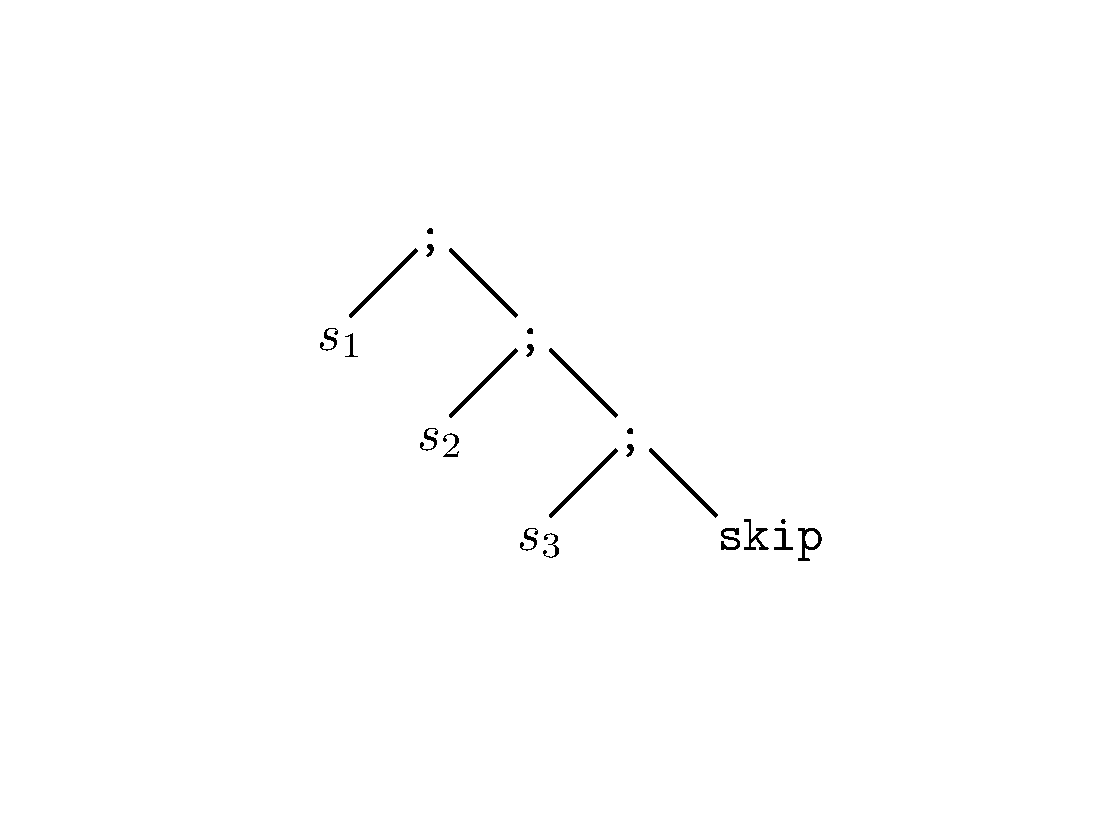
\includegraphics[trim={3cm 3cm 3cm 3cm}, clip, width=6cm]{graphics/rightAssocSkip}
\end{exmp}
These assumptions highly simplify reasoning about statements.


\subsection{Static Semantics}
\label{sec:static-semantics}
% AXIOMATIC
The static semantics of \svl consist of typing rules and a Hoare calculus making use of those typing rules.
All the rules are implicitly parameterized over some program $p \in \setProgram$, necessary for example to extract the type of a field in the following typing rules.

\begin{figure}[h]
    \boxed{\sType{\Gamma}{e}{T}}
    %% Inductive Semantics.hasStaticType
\begin{mathpar}
\inferrule* [Right=STValNum]
{
    ~
}
{
    \sType {\Gamma} {\ev{${{n}}$}} {\Tint}
}
\end{mathpar}

\begin{mathpar}
\inferrule* [Right=STValNull]
{
    ~
}
{
    \sType {\Gamma} {\ev{${\enull}$}} {{C}}
}
\end{mathpar}

\begin{mathpar}
\inferrule* [Right=STVar]
{
    {\Gamma(x)} = {{T}}
}
{
    \sType {\Gamma} {\ex{${x}$}} {T}
}
\end{mathpar}

\begin{mathpar}
\inferrule* [Right=STField]
{
    \sType {\Gamma} {e} {{C}} \\
    {\fieldType({C}, {f})} = {{T}}
}
{
    \sType {\Gamma} {\edot{${e}$}{${f}$}} {T}
}
\end{mathpar}


% Inductive Semantics.hasStaticType
\begin{mathpar}
\inferrule* [right=STValNum]
{
    ~
}
{
    \sType {\Gamma} {\ev{${{n}}$}} {\Tint}
}

\inferrule* [right=STValNull]
{
    ~
}
{
    \sType {\Gamma} {\ev{${\enull}$}} {{C}}
}

\inferrule* [right=STVar]
{
    {\Gamma(x)} = {{T}}
}
{
    \sType {\Gamma} {\ex{${x}$}} {T}
}

\inferrule* [right=STField]
{
    \sType {\Gamma} {e} {{C}} \\
    {\fieldType({C}, {f})} = {{T}}
}
{
    \sType {\Gamma} {\edot{${e}$}{${f}$}} {T}
}
\end{mathpar}


    \caption{\svl: Static Typing of Expressions}
\end{figure}

\begin{figure}[h!]
    \boxed{\thoare {\Gamma} {\phi_{pre}} {\overline{s}} {\phi_{post}}}
    % Inductive Semantics.hoare
\begin{mathpar}
\inferrule* [Right=HAlloc]
{
    {\phi} \implies {\phi'} \\
    {\emptyset} \sfrmphi {\phi'} \\
    {x} \not \in {FV(\phi')} \\
    {\Gamma} \vdash {\ex{${x}$}} : {{C}} \\
    {\fields({C})} = {{\overline{f}}}
}
{
    {\Gamma} \hoare {\phi} {{\sAlloc {${x}$} {${C}$}}} {\phiCons{${\phi'}$}{${\phiCons{${\phiNeq {${\ex{${x}$}}$} {${\ev{${\vnull}$}}$}}$}{${\overline{\acc({x}, f_i)}}$}}$}}
}
\end{mathpar}

\begin{mathpar}
\inferrule* [Right=HFieldAssign]
{
    {\phi} \implies {\phiCons{${\phiAcc {${\ex{${x}$}}$} {${f}$}}$}{${\phi'}$}} \\
    {\emptyset} \sfrmphi {\phi'} \\
    {\Gamma} \vdash {\ex{${x}$}} : {{C}} \\
    {\Gamma} \vdash {\ex{${y}$}} : {T} \\
    \vdash {C}.{f} : {T}
}
{
    {\Gamma} \hoare {\phi} {{\sFieldAssign {${x}$} {${f}$} {${y}$}}} {\phiCons{${\phi'}$}{${\phiCons{${\phiAcc {${\ex{${x}$}}$} {${f}$}}$}{${\phiCons{${\phiNeq {${\ex{${x}$}}$} {${\ev{${\vnull}$}}$}}$}{${\ensuremath{{\phiEq {${\edot{${\ex{${x}$}}$}{${f}$}}$} {${\ex{${y}$}}$}}}}$}}$}}$}}
}
\end{mathpar}

\begin{mathpar}
\inferrule* [Right=HVarAssign]
{
    {\phi} \implies {\phi'} \\
    {\emptyset} \sfrmphi {\phi'} \\
    {x} \not \in {FV(\phi')} \\
    {x} \not \in {FV({e})} \\
    {\Gamma} \vdash {\ex{${x}$}} : {T} \\
    {\Gamma} \vdash {e} : {T} \\
    {\accFor {{e}}} \subseteq {\phi'}
}
{
    {\Gamma} \hoare {\phi} {{\sVarAssign {${x}$} {${e}$}}} {\phiCons{${\phi'}$}{${\ensuremath{{\phiEq {${\ex{${x}$}}$} {${e}$}}}}$}}
}
\end{mathpar}

\begin{mathpar}
\inferrule* [Right=HReturn]
{
    {\phi} \implies {\phi'} \\
    {\emptyset} \sfrmphi {\phi'} \\
    {\xresult} \not \in {FV(\phi')} \\
    {\Gamma} \vdash {\ex{${x}$}} : {T} \\
    {\Gamma} \vdash {\ex{${\xresult}$}} : {T}
}
{
    {\Gamma} \hoare {\phi} {{\sReturn {${x}$}}} {\phiCons{${\phi'}$}{${\ensuremath{{\phiEq {${\ex{${\xresult}$}}$} {${\ex{${x}$}}$}}}}$}}
}
\end{mathpar}

\begin{mathpar}
\inferrule* [Right=HCall]
{
    {\Gamma} \vdash {\ex{${y}$}} : {{C}} \\
    {\mmethod({C}, {m})} = {{\method {${T_r}$} {${m}$} {${T_p}$} {${z}$} {${\requires {\phi_{pre}};~\ensures {\phi_{post}};}$} {${\_}$}}} \\
    {\Gamma} \vdash {\ex{${x}$}} : {T_r} \\
    {\Gamma} \vdash {\ex{${z'}$}} : {T_p} \\
    {\phi} \implies {\phiCons{${\phiNeq {${\ex{${y}$}}$} {${\ev{${\vnull}$}}$}}$}{${\phiCons{${\phi_p}$}{${\phi'}$}}$}} \\
    {\emptyset} \sfrmphi {\phi'} \\
    {x} \not \in {FV(\phi')} \\
    x \neq y \wedge x \neq z' \\
    {\phi_p} = {{\phi_{pre}}[{y}, {z'} / {\xthis}, {{z}}]} \\
    {\phi_q} = {{\phi_{post}}[{y}, {z'}, {x} / {\xthis}, {{z}}, {\xresult}]}
}
{
    {\Gamma} \hoare {\phi} {{\sCall {${x}$} {${y}$} {${m}$} {${z'}$}}} {\phiCons{${\phi'}$}{${\phi_q}$}}
}
\end{mathpar}

\begin{mathpar}
\inferrule* [Right=HAssert]
{
    {\phi} \implies {\phi'}
}
{
    {\Gamma} \hoare {\phi} {{\sAssert {${\phi'}$}}} {\phi}
}
\end{mathpar}

\begin{mathpar}
\inferrule* [Right=HRelease]
{
    {\phi} \implies {\phiCons{${\phi_r}$}{${\phi'}$}} \\
    {\emptyset} \sfrmphi {\phi'}
}
{
    {\Gamma} \hoare {\phi} {{\sRelease {${\phi_r}$}}} {\phi'}
}
\end{mathpar}

\begin{mathpar}
\inferrule* [Right=HDeclare]
{
    {x} \not\in \dom({\Gamma}) \\
    {{\Gamma}, {x} : {T}} \hoare {\phiCons{${\phiEq {${\ex{${x}$}}$} {${\ev{${\texttt{defaultValue}({T})}$}}$}}$}{${\phi}$}} {\overline{s}} {\phi'}
}
{
    {\Gamma} \hoare {\phi} {{\sDeclare {${T}$} {${x}$}} {\overline{s}}} {\phi'}
}
\end{mathpar}

\begin{mathpar}
\inferrule* [Right=HHold]
{
    {\phi_f} \implies {\phiCons{${\phi_r}$}{${\phi'}$}} \\
    {\phi'} \implies {\phi} \\
    {\Gamma} \hoare {\phi_r} {\overline{s}} {\phi_r'}
}
{
    {\Gamma} \hoare {\phi_f} {{\sHold {${\phi}$} {${\overline{s}}$}}} {\phiCons{${\phi_r'}$}{${\phi'}$}}
}
\end{mathpar}

\begin{mathpar}
\inferrule* [Right=HSeq]
{
    {\Gamma} \hoare {\phi_p} {\overline{s_1}} {\phi_q} \\
    {\Gamma} \hoare {\phi_q} {\overline{s_2}} {\phi_r}
}
{
    {\Gamma} \hoare {\phi_p} {{\overline{s_1}}\ttt{;} {\overline{s_2}}} {\phi_r}
}
\end{mathpar}


    \caption{\svl: Hoare Calculus} 
\end{figure}


%% FRAMING
%% Inductive Semantics.sfrme
\begin{mathpar}
\inferrule* [Right=WFVar]
{
    ~
}
{
    {A} \sfrme {\ex{${x}$}}
}
\end{mathpar}

\begin{mathpar}
\inferrule* [Right=WFValue]
{
    ~
}
{
    {A} \sfrme {\ev{${v}$}}
}
\end{mathpar}

\begin{mathpar}
\inferrule* [Right=WFField]
{
    {({e}, {f})} \in {A} \\
    {A} \sfrme {e}
}
{
    {A} \sfrme {\edot{${e}$}{${f}$}}
}
\end{mathpar}



\subsection{Well-Formedness}
\label{sec:well-formedness}
Apart from checking method contracts, a verifier or compiler may enforce further rules before accepting a program as “well formed”.
For \svlidf we give the rules formalized in figure \ref{fig:idf-wf}.

\begin{figure}[h]
    
\begin{mathpar}
\inferrule* [Right=OkProgram]
{
\overline{cls_i \OK} \\
\thoare {~} {\phiTrue} {s} {\phi}
}
{(\overline{cls_i}~s) \OK}
\end{mathpar}

\begin{mathpar}
\inferrule* [Right=OkClass]
{
\text{unique $field$-names} \\
\text{unique $method$-names} \\
\overline{method_i \OKinC}
}
{(\class {$C$} {$\overline{field_i}$} {$\overline{method_i}$}) \OK}
\end{mathpar}

\begin{mathpar}
\inferrule* [Right=OkMethod]
{
    \thoare {x : T_x, \ethis : C, \eresult : T_m} {\phi_1} {s} {\phi_2} \\\\
    \FV(\phi_1) \subseteq \{ x, \ethis \} \\
    \FV(\phi_2) \subseteq \{ x, \ethis, \eresult \} \\\\
    \sfrmphi \phi_1 \\
    \sfrmphi \phi_2 \\
    \neg \writesTo(s, x)
}
{(\method {$T_m$} {$m$} {$T_x$} {$x$} {\contract {$\phi_1$} {$\phi_2$}} {$s$}) \OKinC}
\end{mathpar}
    \caption{\svlidf: Well-Formedness}
    \label{fig:idf-wf}
\end{figure}

%% OkMethod
The premises of $\tset{OkMethod}$ make sure that reasoning about calls is sound.
As expected, the method contract is checked, while also making sure that it contains self-framing formulas.
Furthermore, the free variables are restricted to those occurring in the method signature.
The following example illustrates why this is necessary.

%% example
\begin{example}{Leaking Postcondition}
\begin{lstlisting}
int identity(int a)
    requires true;
    ensures  (b = 3);
{
    int b;
    b = 3;
    return a;
}
\end{lstlisting}
While the method passes static verification, it could lead to unsound proofs.
Note how \tset{HCall} forwards the postcondition after replacing known variables with their counterparts.
\phiEq{b}{3} is unaffected by this replacement, ending up in the postcondition of the call statement.

Should the call site also know a variable \ttt{b}, then \phiEq{b}{3} will most likely not reflect the state of that variable.
\end{example}

For similar reasons, we prevent writes to the method's parameter.
Changes to the parameter would otherwise end up in the postcondition which is forwarded to the call site.
Information about the formal parameter is then reflected back on the variable passed as actual parameter for the method call.
However, since parameters are passed by value, this information would be false -- the actual parameter will have the same value before and after the method call.


\subsection{Dynamic Semantics}


\section{Deriving a Gradually Verified Language}

\subsection{Gradual Formulas}
% syntax, concretization
% lifting predicates, lifting functions

\subsection{Abstracting Static Semantics}
% non-deterministic static hoare rules make “quality of lifting” reasoning hard! if even {a}...{true} is valid statically, how to express/measure “badness” of emitting {a}...{?}

\subsection{Abstracting Dynamic Semantics}


\chapter{Implementation}
...of \ref{sec:a-statically-verified}

\section{Prepare Hoare Rules}
% make deterministic, split into 3 sections

\subsection{Deterministic Functions}

\section{Gradualize Hoare Rules}

\subsection{Gradualize Functions}
% IDF stuff will probably only show up here!

\section{Enhancing an Unverified Language}


\chapter{Evaluation/Analysis}
> E:
with gradual typestates the same problem happened: as soon as the potential for unknown annotations was accepted, there was a “baseline cost” just to maintain the necessary infrastructure.
With simple gradual types, it’s almost nothing. With gradual effects, we’ve shown that it can boil down to very little (a thread-local variable with little overhead, see OOPSLA’15). 

% relationship LC and verification! which rules are derived by which, correspondence table


\chapter{Conclusion}
Recap, remind reader what big picture was.
Briefly outline your thesis, motivation, problem, and proposed solution.

\section{Limitations}

\section{Future Work}


\chapter{Appendix}


\chapter{UNSORTED}

\section{HoareMotivEx}
\label{sec:hoaremotivex}

% AGT: mention draft about refinement types?

Hoare Logic as formal setting

\begin{verbatim}
class Point
{
    int manhattenDistance(Point p)
        requires \phi_{pre};
        ensures  \phi_{post};
    {
        s1;
        s2;
        .
        .
        .
    }
}
\end{verbatim}

\begin{displaymath}
\thoare
    {\ethis : \type{Point}, \ex{p} : \type{Point}, \eresult : \Tint}
    {\phi_{pre}}
    {s1; s2; ...}
    {\phi_{post}}
\end{displaymath}

\section{MotivationExamples}
\label{sec:motivationexamples}

\subsection{Argument Validation}
The following Java example motivates the use of verification for argument validation.
\begin{lstlisting}
boolean hasLegalDriver(Car c)
{
    // business logic:
    resAllocate();
    boolean result = c.driver.age >= 18;
    resFree();
    return result;
}
\end{lstlisting}
A call to \ttt{hasLegalDriver} fails if \ttt{c} or \ttt{c.driver} evaluate to \ttt{null}.
Note that, although the Java runtime has defined behavior in to those cases (throwing an exception), we might still have created a resource leak.
To prevent this from happening, arguments have to be validated before entering the business logic.
\begin{lstlisting}
boolean hasLegalDriver(Car c)
{
    if (!(c != null))
        throw new IllegalArgException("expected c != null");
    if (!(c.driver != null))
        throw new IllegalArgException("expected c.driver != null");
        
    // business logic (requires 'c.driver.age' to evaluate)
}
\end{lstlisting}

Note that these runtime checks dynamically verifies a method contract, having \ttt{c != null \&\& c.driver != null} as precondition.
Naturally, the drawbacks of dynamic verification apply:
Violations of the method contract are only detected at runtime, possibly go unnoticed for a long time and impose a runtime overhead which might not be acceptable in all scenarios.
Java even has dedicated assertion syntax simplifying dynamic verification:
\begin{lstlisting}
boolean hasLegalDriver(Car c)
{
    assert c != null;
    assert c.driver != null;

    // business logic (requires 'c.driver.age' to evaluate)
}
\end{lstlisting}
Note however that such assertions are dropped from regular builds, meaning that the method contract is no longer verified!

With support of additional tools, a more declarative approach is possible using JML syntax:
\begin{lstlisting}
//@ requires c != null && c.driver != null;
boolean hasLegalDriver(Car c)
{
    // business logic (requires 'c.driver.age' to evaluate)
}
\end{lstlisting}

There are two basic ways to turn this annotation into a guarantee:
\begin{description}
    \item[Static Verification (e.g. ESC/Java, see \cite{leino2000esc})]~\\
    Verification will only succeed if the precondition is provable at all call sites.
    This is achievable in two ways:
    \begin{itemize}
        \item
        Rigorously annotate the call sites, guiding the verifier towards a proof.
        \item 
        Add parameter validation to the call sites, effectively duplicating the original runtime check across the program.
        Note that this approach combines static and dynamic validation in order to get a performance benefit (no more runtime checks required where precondition was provable) and circumvent rigorous annotation.
        The drawback is of course code duplication.
    \end{itemize}
    % benefits, drawbacks
    
    %There are obvious limitations to this approach, static verification tends to be invasive.
    %At least there is a performance benefit: 
    %Runtime checks (originally part of every call) are now only necessary in places where verification would not succeed otherwise.
    
    \item[Dynamic Verification (e.g. run JML4c, see \cite{sarcar2010new}]~\\
    This approach basically converts the annotation back into a runtime check equivalent to our original argument validation.
    % benefits, drawbacks
\end{description}

Gradual verification would pursue the combined approach without (visible) code duplication:
Static verification is used where possible, dynamic verification where needed.
Note that for the programmer this means that adding the method contract comes with no further obligations.

\subsection{Limitations of Static Verification}
The following example is written in a Java-like language with dedicated syntax for method contracts (similar to Eiffel and Spec\#).
We assume that this language is statically verified, i.e. static verification is part of the compilation.

The example shows the limitations of static verification using the Collatz sequence as an algorithm too complex to describe concisely in a method contract:
\begin{lstlisting}
int collatzIterations(int iter, int start)
    requires 1 <= start;
    ensures  1 <= result;
{
    // ...
}

int myRandom(int seed)
    requires 1 <= seed   && seed   <= 10000;
    ensures  1 <= result && result <= 3;     // not provable
{
    int result = collatzIterations(300, seed);
    // we know:        result $\in$ { 1, 2, 4 }
    // verifier knows: 1 <= result
    
    if (result == 4) result = 3;
    return result;
}
\end{lstlisting}
The first method \ttt{collatzIterations} iterates given number of times, starting at given value.
We assume that the only provable contract is that positive start value results in positive result.
The second method \ttt{myRandom} uses the Collatz sequence to generate a pseudo random number from given seed.
It is known to the programmer that start values up to 10000 result in convergence of the sequence after 300 iterations.
After mapping 4 to 3, we are thus given a number between 1 and 3, as described in the postcondition.

Unfortunately, the verifier cannot deduce this fact since the postcondition of \ttt{collatzIterations} only guarantees positive result, but no specific range of values.
Again, we can resort to dynamic methods to aid verification:

\begin{lstlisting}
...
{
    int result = collatzIterations(300, seed);
    // we know:        result $\in$ { 1, 2, 4 }
    // verifier knows: 1 <= result
    
    // knowledge "cast"
    if (!(result <= 4))
        throw new IllegalStateException("expected result <= 4");

    // verifier knows: 1 <= result && result <= 4 
    
    if (result == 4) result = 3;
    return result;
}
\end{lstlisting}

This solution is not satisfying as it required additional work by the programmer to convince the verifier.
Furthermore, the solution is in an unintuitive location:
The problem is not caused by \ttt{myRandom}, yet it is solved there.
The actual problem is that the postcondition of \ttt{collatzIterations} is too weak, causing the verifier to fail deducing our knowledge.

Gradual verification allows enhancing the postcondition with “unknown” knowledge that can be reinterpreted arbitrarily, adding appropriate runtime checks to guarantee that this reinterpretation was in fact valid:
\begin{lstlisting}
int collatzIterations(int iter, int start)
    requires 1 <= start;
    ensures  1 <= result && ?;
{
    // ...
}

int myRandom(int seed)
    requires 1 <= seed   && seed   <= 10000;
    ensures  1 <= result && result <= 3;
{
    int result = collatzIterations(300, seed);
    // we know: result $\in$ { 1, 2, 4 }
    
    // verifier allowed to
    //  assume 1 <= start && result <= 4
    //  from   1 <= start && ?
    // (adding runtime check)
    
    if (result == 4) result = 3;
    return result;
}
\end{lstlisting}
Note the \ttt{?} in the postcondition of \ttt{collatzIterations}.

% gradual:
% - not in a sense of GraVy
% - assertions are GUARANTEED not to be violated (analogous to type safety of gradually typed languages), meaning that
%    - as much as possible is verified statically
%    - if necessary, (ideally: as few as possible) dynamic checks kick in
% - full continuum between static and dynamic

% static checking
% dynamic checking
% combine static and dynamic checking
% views:
% - add designated "?" to statically checked language, making checking optional
% - introduce checking to unchecked language, making "?" the default value
% typing
% transition to verification
% - of particular interest, cause limitations due to syntax or decidability make full checking impossible,
%    possibly making use of static verification impossible and the program thus unverifiable
%    inevitable incompleteness of static verifiers!
%    GraVy: measure, only \textit{classifies} code into sections: correctness statically guaranteed, correctness statically disproved, no static guarantee so far

% very desirable in practice
% gradual version of a language is inherently a strict superset of original language
% 

% our approach allows extension of existing languages (without any verification) by adding transpilation step

% why would you want continuum?
% - move toward satically verified program without giving up guarantees!
% - while "barely typed" languages hardly make sense, programs with "little verification" are already highly useful
%    i.e. verification even makes sense as "rarely used feature"!
%    ArgumentException-example
%    -    performance benefit!
%    -    cleaner code!
%    -    makes more sense semantically
% having optional types 

% Future Work:
% implement on top of existing languages
% - tracking access via ThreadLocalStorage
% - transpilation (e.g. C# Roslyn compiler extension)
